\documentclass[12pt]{article}
\usepackage{graphicx,psfrag,amsfonts,float,mathbbol,xcolor,cleveref}
\usepackage{arydshln}
\usepackage{amsmath}
\usepackage{subfiles}
\usepackage{tikz}
\usepackage[mathscr]{euscript}
\usepackage{enumitem}
\usepackage{accents}
\usepackage{framed}
\usepackage{subcaption}

\usepackage{natbib}
\usepackage{mathtools}
\usepackage{IEEEtrantools}
\usepackage{times}
\usepackage{arydshln}
\usepackage{cite}
\usepackage{amsthm}
\usepackage[letterpaper, left=1in, top=1in, right=1in, bottom=1in,nohead,includefoot, verbose, ignoremp]{geometry}
\newcommand\numberthis{\addtocounter{equation}{1}\tag{\theequation}}
\newcommand*\needsparaphrased{\color{red}}
\newcommand*\needscited{\color{orange}}
\newcommand*\needsproof{\color{blue}}
\newcommand*\outlineskeleton{\color{green}}
\newcommand{\ms}{\scriptscriptstyle}
\newcommand{\hilbert}{\mathcal{H}}
\newcommand{\hilbertl}{\mathcal{H}_{\langle l \rangle}}
\newcommand{\hilbertm}{\mathcal{H}_{\langle m \rangle}}
\newcommand{\hilbertlnull}{\mathcal{H}_{0\langle l \rangle}}
\newcommand{\hilbertmnull}{\mathcal{H}_{0\langle m \rangle}}
\newcommand{\hilbertlpen}{\mathcal{H}_{1\langle l \rangle}}
\newcommand{\hilbertmpen}{\mathcal{H}_{1\langle m \rangle}}
\newcommand{\PP}{\mathcal{P}}
\newcommand{\vphistar}{\mbox{\boldmath $\phi$}}
\newcommand{\vsigmasq}{\mbox{\boldmath $\sigma^2$}}
\newcommand{\bfeps}{\mbox{\boldmath $\epsilon$}}
\newcommand{\bfgamma}{\mbox{\boldmath $\gamma$}}
\newcommand{\bflam}{\mbox{\boldmath $\lambda$}}
\newcommand{\bfphi}{\mbox{\boldmath $\phi$}}
\newcommand{\bfsigma}{\mbox{\boldmath $\sigma$}}
\newcommand{\bfbeta}{\mbox{\boldmath $\beta$}}
\newcommand{\bfalpha}{\mbox{\boldmath $\alpha$}}
\newcommand{\bfe}{\mbox{\boldmath $e$}}
\newcommand{\bff}{\mbox{\boldmath $f$}}
\newcommand{\bfone}{\mbox{\boldmath $1$}}
\newcommand{\bft}{\mbox{\boldmath $t$}}
\newcommand{\bfo}{\mbox{\boldmath $0$}}
\newcommand{\bfO}{\mbox{\boldmath $O$}}
\newcommand{\bfx}{\mbox{\boldmath $x$}}
\newcommand{\bfX}{\mbox{\boldmath $X$}}
\newcommand{\bfz}{\mbox{\boldmath $z$}}
\newcommand{\tildeY}{\tilde{Y}}
\newcommand{\tildey}{\tilde{y}}
\newcommand{\tildeQ}{\tilde{Q}}
\newcommand{\tildeR}{\tilde{R}}
\newcommand{\tildeA}{\tilde{A}}
\newcommand{\tildeepsilon}{\tilde{\epsilon}}
\newcommand{\bftheta}{\mbox{\boldmath $\theta$}}
\newcommand{\bfepsilon}{\mbox{\boldmath $\epsilon$}}
\newcommand{\tildeS}{\tilde{S}}

\newcommand{\bfm}{\mbox{\boldmath $m}}
\newcommand{\bfy}{\mbox{\boldmath $y$}}
\newcommand{\bfa}{\mbox{\boldmath $a$}}
\newcommand{\bfb}{\mbox{\boldmath $b$}}
\newcommand{\bfY}{\mbox{\boldmath $Y$}}
\newcommand{\bfS}{\mbox{\boldmath $S$}}
\newcommand{\bfZ}{\mbox{\boldmath $Z$}}
\newcommand{\cardT}{\vert \mathcal{T} \vert}
%\newenvironment{theorem}[1][Theorem]{\begin{trivlist}
%\item[\hskip \labelsep {\bfseries #1}]}{\end{trivlist}}
%\newenvironment{corollary}[1][Corollary]{\begin{trivlist}
%\item[\hskip \labelsep {\bfseries #1}]}{\end{trivlist}}
%\newenvironment{proposition}[1][Proposition]{\begin{trivlist}
%\item[\hskip \labelsep {\bfseries #1}]}{\end{trivlist}}
%\newenvironment{definition}[1][Definition]{\begin{trivlist}
%\item[\hskip \labelsep {\bfseries #1}]}{\end{trivlist}}

\newtheorem{theorem}{Theorem}[section]
\newtheorem{lemma}[theorem]{Lemma}
\newtheorem{proposition}[theorem]{Proposition}
\newtheorem{corollary}[theorem]{Corollary}

\theoremstyle{definition}
\newtheorem{definition}{Definition}[section]
\newtheorem{example}{Example}[section]
\def\bL{\mathbf{L}}

\begingroup\lccode`~=`_
\lowercase{\endgroup\def~}#1{_{\scriptscriptstyle#1}}
\AtBeginDocument{\mathcode`_="8000 \catcode`_=12 }

\makeatletter
\renewcommand{\theenumi}{\Roman{enumi}}
\renewcommand{\labelenumi}{\theenumi.}
\renewcommand{\theenumii}{\Alph{enumii}}
\renewcommand{\labelenumii}{\theenumii.}
\renewcommand{\p@enumii}{\theenumi.}
\makeatother

\begin{document}

%\nocite{*}
\def\bL{\mathbf{L}}
%\usepackage{mathtime}

%%UNCOMMENT following line if you have package


\title{ Nonparametric Covariance Estimation for Longitudinal Data via Penalized Tensor Product Splines}

\author{Tayler A. Blake\thanks{The Ohio State University, 1958 Neil Avenue, Columbus, OH 43201} \and  Yoonkyung Lee\thanks{The Ohio State University, 1958 Neil Avenue, Columbus, OH 43201}}

\bibliographystyle{plainnat}
\maketitle

\section{Smoothing Spline Varying-coefficient Models for Covariance Estimation}

A predominant difficulty in the estimation of covariance matrices is the potentially high dimensionality of the problem, as the number of unknown elements in the covariance matrix grows quadratically with the size of the matrix. It is well-known that the sample covariance matrix can be unstable in high dimensions; ways for controlling the complexity of estimates is highly desirable for improving stability of estimates. In the longitudinal-data literature, it is a common practice to use parametric models for the covariance structure.  Many have specified parsimonious parametric models for $\phi_{ijk}$ to overcome the issue of dimensionality.  

\bigskip

We naturally accommodate irregularly spaced data and unequal sample sizes between subjects by defining the autoregressive parameters as the values of a smooth function evaluated at within-subject pairs of observed time points.  Furthermore, by viewing $\phi\left(t,s\right)$ as a smooth \emph{bivariate} function, we can utilize the information across the subdiagonals of $T$ to inform the fit, rather than treating each subdiagonal separately.  As in the classical nonparametric function estimation setting, we assume $\phi$ to vary in a high-dimensional (possibly infinite) function space. We propose two representations of $\phi\left(\cdot, \cdot\right)$ and $\sigma\left(\cdot, \cdot\right)$: approximation by smoothing splines and approximation by B-spline basis expansion. 

We assume $Y\left(t\right)$ has covariance function $G\left(t,s\right)$ and that $\epsilon\left(t\right)$ follows a zero mean Gaussian white noise process with unit variance. Under mild assumptions regarding the behaviour of $Y$, then $G\left(t,s\right)$ satisfies some smoothness conditions, where smoothness is defined in terms of square integrability of certain derivatives. We view the entries of $\Sigma$ as values of $G$ evaluated at the distinct pairs of within-subject observed time points. 
\bigskip


If we consider the Cholesky decomposition of $\Sigma$ within such functional context, it is natural to extent the same notion to the elements of $T$ and $D$. We view the GARPs $\lbrace \phi_{tj} \rbrace$ and innovation variances as the evaluation of the smooth functions $\tilde{\phi}\left(t,s\right)$ and $\sigma^2\left(t\right)$ at observed time points, which we assume  are drawn from some distribution having compact domain $\mathcal{T}$. Without loss of generality, we take $\mathcal{T} = \left[0,1\right]$. Henceforth, we view $\tilde{\phi}$ and $\sigma^2$ as a smooth continuous functions, but for ease of exposition, we let $\tilde{\phi}_{ij}$ denote the varying coefficient function evalutated at $\left(t_i,t_j\right)$: 
\[
\tilde{\phi}_{tj} = \tilde{\phi}\left(t_{i},t_{j}\right). 
\]
Adopting similar notation for the innovation variance function, denote
\[
\sigma_{j}^2 = \sigma^2\left(t_{j}\right),
\]
where $0 \le t_{j} < t_{i} \le 1$ for $j < i$. This leads to varying coefficient model

\begin{equation}  \label{eq:cholesky-regression-model-1} 
y\left(t_{i} \right)  = \sum_{j=1}^{i-1} \tilde{\phi}\left(t_{i} ,t_{j}\right) y\left(t_{j}\right) + \sigma\left(t_{j}\right)\epsilon\left({t_j}\right) \;\;\;\; i=1,\dots, M, 
\end{equation}
\noindent

Our goal is now to estimate the above model, utilizing bivariate smoothing to estimate $\tilde{\phi}\left(t,s\right)$ for $0 \le s < t \le 1$,  and one-dimensional smoothing to estimate $\sigma\left(t \right)$, $0 \le t \le 1$. Our proposed method for covariance estimation defines a flexible, general framework which makes all of the existing techniques for penalized regression accessible for the seemingly far different task of estimating a covariance matrix.

\bigskip

Our approach to estimation is constructed to provide a fully data-driven methodology for selecting the optimal covariance model (given some optimization criterion) from a expansive class of estimators ranging in complexity from that of the previously aforementioned parametric models to that of completely unstructured estimators, like the sample covariance matrix. We leverage the collection of regularization techniques that are accessible in the usual function estimation setting. By properly specifying the roughness penalty, our optimization procedure results in null models which correspond to the parametric and semiparametric models for $\phi$ and $\sigma^2$ discussed in \ref{chapter-1-parametric-semiparametric-garp-models}. To facilitate the penalty specification that achieves this, we consider modeling the varying coefficient function which takes inputs

\begin{align} 
\begin{split}\label{eq:l-m-transformation}
l &= t - s \\
m &= \frac{t + s}{2}, \\
\end{split}
\end{align}
\noindent
 where $l$ is the continuous analogue of the usual ``lag'' between time points $t$ and $s$, and $m$ is simply its orthogonal direction. We have discussed many parsimonious covariance structures which model $y\left(t\right)$ as a stationary process with covariance function which depends on time points $t_i$ and $t_j$ only through the Euclidean distance $\vert \vert t_i - t_j \vert \vert$ between them. Covariance functions taking the form $Cov\left(y\left( t_i \right),y\left( t_j \right)\right) =G\left(t_i,t_j\right) = G\left(\vert \vert t_i - t_j \vert \vert \right)$ can then be written as 

\begin{equation*}
Cov\left(y\left( t_i \right),y\left( t_j \right)\right) = G\left( l_{ij}  \right)
\end{equation*}
\noindent
where $l_{ij} =  \vert  t_i - t_j  \vert $. Regularizing the functional components of the Cholesky decomposition so that functions incurring large penalty correspond to functions which vary in only $l$ and are constant in $m$ allows us to model nonstationarity in a fully data-driven way.  Our goal is to estimate

\begin{equation} 
\phi\left(l,m\right) = \phi\left(s-t, \frac{1}{2}\left(s+t\right)\right) = \tilde{\phi}\left(t,s\right).
\end{equation}

\bigskip

While our framework allows for estimation of the autoregressive coefficient function and the innovation variance function via any nonparametric regression setup, we focus on two primary approaches for representing $\phi$ and $\sigma$. First, we assume that $\phi$ belongs to a reproducing kernel Hilbert space, $\mathcal{H}$ and employ the smoothing spline methods of Kimeldorf and Wahba (see \citet{kimeldorf1971some} and \citet{wahba1990spline} for comprehensive presentation.)  To enhance the statistical interpretability of model parameters, we decompose $\phi$ into functional components similar to the notion of the main effect and the interaction terms in classical analysis of variance. We adopt the smoothing spline analogue of the classical ANOVA model proposed by Gu \citet{gu2013smoothing}, and estimation is achieved through similar computational strategies.

\subsection{Penalized maxiumum likelihood estimation of $\phi$, $\log\sigma^2$}

Let random vector $Y$ follow a multivariate normal distribution with zero mean vector and covariance $\Sigma$. The loglikelihood function $\ell \left( Y, \Sigma \right)$ satisfies

\begin{equation} \label{eq:loglik-general-form}
-2\ell\left( Y, \Sigma \right) = \log \vert \Sigma \vert + Y' \Sigma Y
\end{equation}
\noindent
Using $T \Sigma T' = D$, we can write 
\[
\vert \Sigma\vert = \vert D \vert = \prod_{i = 1}^m \sigma_i^2
\]
and 
\[
\Sigma^{-1} = T' D^{-1} T.
\]
Writing \ref{eq:loglik-general-form} in terms of the prediction errors and their variances of the non-redundant entries of $\left(T , D\right)$, we have

\begin{align}
\begin{split} \label{eq:loglik-cholesky-form}
-2\ell\left( Y, \Sigma \right) &= \log \vert D \vert + Y' T' D^{-1} T Y \\
&= \sum_{i = 1}^m \log \sigma_i^2  + \sum_{i = 1}^m \frac {\epsilon_i^2}{\sigma_i^2},
\end{split}
\end{align}
\noindent
where 
\begin{equation} \label{eq:loglik-cholesky-form}
\epsilon_i = \left\{\begin{array}{lr}y\left(t_1\right), & i = 1, \\
y\left(t_i\right) - \sum_{j = 1}^{i-1} \phi\left(v_{ij}\right) y_j, & i= 2, \dots, M, \\
\end{array} \right.
\end{equation}
\noindent
where $\phi\left(v_{ij}\right) = \phi\left(l_{ij},m_{ij}\right) = \tilde{\phi}\left(t_i,t_j\right)$.  Accommodating subject-specific sample sizes and measurement times merely requires appending an additional index to observation times. Let  $Y_1, \dots, Y_N$ denote a sample of $N$ independent mean zero random trajectories from a  multivariate normal distribution with common covariance $\Sigma$. We associate with each trajectory $Y_i = \left(y_{i1}, \dots, y_{i,m_i}\right)'$ with a vector of potentially subject-specific observation times $\left(t_{i1}, \dots, t_{i,m_i}\right)'$, so that the $j^{th}$ measurement of trajectory $i$ is modeled

\begin{align}
\begin{split} \label{eq:cholesky-regression-model-2} 
y\left(t_{ij} \right)  &= \sum_{k=1}^{j-1} \tilde{\phi}\left(t_{ij} ,t_{ik}\right) y\left(t_{ik}\right) + \sigma\left(t_{ij}\right)\epsilon\left(t_{ij}\right)  \\
&= \sum_{k=1}^{j-1} \phi\left(v_{ijk}\right) y\left(t_{ik}\right) + \sigma\left(t_{ij}\right)\epsilon\left(t_{ij}\right)
\end{split}
\end{align}
\noindent
for $i = 1,\dots, N$, $j = 2,\dots, m_i$.
\noindent
Making similar ammendments to indexing, the joint log likelihood for the sample $Y_1, \dots, Y_N$ is given by  

\begin{equation} \label{eq:joint-loglik}
-2\ell\left( Y_1,\dots, Y_N, \phi, \sigma^2 \right) = \sum_{i = 1}^N \sum_{j = 1}^{m_i} \log \sigma_{ij}^2  + \sum_{i = 1}^N \sum_{j = 1}^{m_i} \frac {\epsilon_{ij}^2}{\sigma_{ij}^2},
\end{equation}

\bigskip

With this, we can estimate $\phi$ and $\log\sigma^2$ using maximum likelihood or any of its penalized variants by appending a roughness penalty (penalties) to \ref{eq:joint-loglik}. Employing regularization, we take $\phi$, $\sigma^2$ to minimize 

\begin{equation} \label{eq:penalized-joint-loglik}
-2\ell\left( Y_1,\dots, Y_N, \phi, \sigma^2 \right) +    \lambda J\left( \phi \right) +  \breve{\lambda}\breve{J}\left( \sigma^2 \right),
\end{equation}
\noindent
where $J$ and $\breve{J}$ are roughness penalties on $\phi$ and $\sigma^2$, and $\lambda$, $\breve{\lambda}$ are non-negative smoothing parameters.  To jointly estimate the GARP function and the IV function, we adopt an iterative approach in the spirit of \citet{huang2006covariance}, \citet{huang2007estimation}, and \citet{pourahmadi2000maximum}. A procedure for minimizing \ref{eq:joint-loglik} starts with initializing $\left\{\sigma^2_{ij}\right\} = 1$ for $i = 1,\dots, N$, $j = 1,\dots, m_i$.  For fixed $\sigma^2$, the penalized likelihood (as a function of $\phi$) is given by

\begin{equation} \label{eq:penalized-joint-loglik-given-sigma}
-2\ell_\phi + \lambda J\left(\phi\right) = \sum_{i=1}^N \sum_{j=2}^{m_i} \sigma^{-2}_{ij}\left( y_{ij} - \sum_{k<j} \phi\left(v_{ijk}\right) y_{ik}  \right)^2 + \lambda J\left( \phi \right),
\end{equation}
\noindent
which corresponds to the usual penalized least squares functional encountered  in the nonparametric function estimation literature. The first term, the residual sums of squares, encourages the fitted function's fidelity to the data. The second term penalizes the roughness of $\phi$, and $\lambda$ is a smoothing parameter which controls the tradeoff between the two conflicting concerns. Given $\phi^*$ the minimizer of \ref{eq:penalized-joint-loglik-given-sigma} and setting $\phi = \phi^*$, we update our estimate of $\sigma^2$ by minimizing 

\begin{equation} \label{eq:penalized-joint-loglik-given-phi}
-2\ell_{\sigma^2} + \breve{\lambda} \breve{J}\left(\sigma^2\right) = \sum_{i=1}^N \sum_{j=2}^{m_i} \log \sigma^2_{ij} + \sum_{i=1}^N \sum_{j=1}^{m_i} \sigma_{ij}^{-2} {r_{ij}^*}^2 + \breve{\lambda} \breve{J}\left(\sigma^2 \right),
\end{equation}
where the $\left\{{r_{ij}^*}^2  =\left( y_{ij} - \sum_{k<j} \phi^*\left(v_{ijk}\right) y_{ik}  \right)\right\}$ denote the working residuals based on the current estimate of $\phi$. This process of iteratively updating $\phi^*$ and ${\sigma^2}^*$ is repeated until convergence is achieved. 
\bigskip

The remainder of the chapter is reserved for presenting two functional representations of $\left(\phi, \sigma^2\right)$. The first leverages the rich theoretical foundation of reproducing kernel Hilbert space techniques for function estimation. This framework has been studied extensively for the problem of estimating a function nonparametrically (see \citet{aronszajn1950theory}, \citet{wahba1990spline}, and \citet{berlinet2011reproducing} for detailed examinations), but to our knowledge has received little attention in the context of covariance models. We use a smoothing spline ANOVA decomposition of the varying coefficient function $\phi$ to construct a flexible class of covariance models while simultaneously maintaining interpretability. The second approach is based on the penalized B-splines, or P-splines, of \citet{eilers1996flexible}; these models exhibit many of the attractive numerical properties of the basis functions on which they are built. The formulation of the penalty is independent of the basis, which provides added modeling flexibility due to the ease with which one can employ various types of regularization.

%%%%%%%%%%%%%%%%%%%%%%%%%%%%%%%%%%%%%%%%%%%%%%%%%%%%%%%%%%%%%%%%%%%%%%%%%%%%%%%%%%%%%%%%%%
%%%%%%%%%%%%%%%%%%%%%%%%%%%%%%%%%%%%%%%%%%%%%%%%%%%%%%%%%%%%%%%%%%%%%%%%%%%%%%%%%%%%%%%%%%


\subsection{Smoothing spline representation of $\phi$, $\sigma$}


\subsubsection{An RKHS framework for estimating $\phi$}
\subfile{chapter-2-subfiles/chapter-2-smoothing-spline-representation}


\subsubsection{Example: $m^{th}$ order Sobolev space, $W_m\left(0,1\right)$}
\subfile{chapter-2-subfiles/chapter-2-smoothing-spline-reproducing-kernel-example-1}


\subsubsection{Smoothing parameter selection}
\subfile{chapter-2-subfiles/chapter-2-smoothing-spline-solution}



\subsubsection{An RKHS framework for estimating $\log \sigma^2$}
\subfile{chapter-2-subfiles/chapter-2-iv-smoothing-spline-representation}





%==============================================================================================================================================




%and 
%\begin{equation} \label{eq:loglik-phi-component}
%\sum_{i = 1}^N \sum_{j = 2}^{m_i} \frac{\epsilon_{ij}^2}{\sigma_{ij}^{2}}
%\end{equation}
%
%\begin{equation} \label{eq:loglik-sigma-component}
%\sum_{ \bigcup t_{i1}}  \log \sigma_{i1}^2 + \sum_{i = 1}^N \frac{\epsilon_{i1}^2}{\sigma_{i1}^2}. 
%\end{equation}
%\noindent
%and 
%\begin{equation} \label{eq:loglik-phi-component}
%\sum_{ \bigcup \limits_{k>1} t_{ik}}  \log \sigma_{ij}^2 + \sum_{i = 1}^N \sum_{j = 2}^{m_i} \sigma_{ij}^{-2}  \left( y_{ij} - \sum \limits_{k < j}\phi_{ijk} y_{ik} \right)^2 .
%\end{equation}


%==============================================================================================================================================
%==============================================================================================================================================

\subsection{A B-spline representation for pp functions}

\subfile{chapter-2-subfiles/chapter-2-bspline-representation}


%==============================================================================================================================================

\subsection{Single-regressor varying coefficient models via B-spline basis expansions}

\subfile{chapter-2-subfiles/chapter-2-bspline-single-index-vc-models}

%==============================================================================================================================================

%%==============================================================================================================================================
%%==============================================================================================================================================
%%==============================================================================================================================================


\subsection{P-spline estimators for regularized estimation of fitted curves}

\subfile{chapter-2-subfiles/chapter-2-pspline-models-intro}

 %%==============================================================================================================================================
 
 \subsubsection{Difference penalties}
 \subfile{chapter-2-subfiles/chapter-2-pspline-difference-penalties}

%==============================================================================================================================================


\subsubsection{P-splines for single-index VC models}
 \subfile{chapter-2-subfiles/chapter-2-single-index-pspline-vc-models}

%%====================================================================================

\subsection{Properties of P-splines}
 \subfile{chapter-2-subfiles/chapter-2-properties-of-psplines}


%%====================================================================================
\subsection{The reguarlized MLE for $\phi$ via tensor product P-splines}
 \subfile{chapter-2-subfiles/chapter-2-tensor-product-pspline-MLE}


%We employ maximum likelihood  for the estimation of  the varying coefficient function $\phi\left(t,s\right)$ and the innovation variance function $\sigma\left(t\right)$, though neither the derivation the form of model~\ref{eq:ARmodel} nor model~\ref{eq:MyModel} via the Cholesky decomposition rely on any assumptions about the distribution of $Y$. 
%
%For fixed $\left\{ \sigma_j^2 \right\}$, as a function of $\phi_{jk}$ the negative log-likelihood for a sample of $N$  i.i.d. observations $Y_1,Y_2,\dots,Y_N$ from a multivariate Gaussian distribution is proportional to the usual error sums of squares:
%
%\begin{equation}
%-2 L\left(y_1,\dots,y_N ,\phi \vert \vsigmasq \right) \propto \sum_{i=1}^N \sum_{j=2}^{m_i} \sigma\left({t_j}\right)^{-2} \left(y_{ij} - \sum_{k=1}^{j-1}\phi\left({t_{ij},t_{ik}}\right)y_{ik} \right)^2 \label{loglikelihood}
%\end{equation}
%\noindent
%where 
%\[
%y_i = \left( y_{i1}, y_{i2}, \dots, y_{i,m_i}\right), \quad i=1,\dots,N 
%\] 
%
%%% explain here that we omit y_{i1} from the likelihood here because in the first stage of estimation (for $\phi$), the first observation in each vector doesn't contribute to the likelihood
%\noindent
%denotes the vector of observations for subject $i$ with corresponding measurement times 
%\[
%t_{i1} < t_{i2} < \dots < t_{i,m_i}.
%\]
%The form of the likelihood of $y_1,\dots,y_N$ indicates that we allow both the number of measurements as well as the observation times to varying across subjects. The $\left\{t_{ij} \right\}$ need not be evenly-spaced within or across individuals. Denote the innovation variance function evaluated at the vector of observed time points by $\vsigmasq$, and similarly let $\vphistar$ denote the resulting vector when evaluating $\phi$ at the observed grid of time points, transformed to the $l$-$m$ axis. Estimation of the varying coefficient function and the innovation variance function may be accomplished in an iterative fashion:
%
%\fbox{\parbox{\textwidth}{\begin{enumerate}
%\item Fix $\vsigmasq = \vsigmasq_0$;
%\item find $\widehat{\vphistar} = \underset{\vphistar}{\arg\max} -2 L\left(y_1,\dots,y_N ,\vphistar \vert \vsigmasq_0 \right)$.
%\item Fix $\vphistar= \widehat{\vphistar}$;
%\item find $\widehat{\vsigmasq} = \underset{\vsigmasq}{\arg\max} -2 L\left(y_1,\dots,y_N , \vsigmasq \vert \widehat{\vphistar} \right)$.
%\item Iterate until convergence.
%\end{enumerate}}}
%
%\vspace{0.5cm}


% 
%\section{\emph{Penalized maximum likelihood estimation}}
%
%\begin{enumerate}
%\item Fix $\sigma_{ij}^2 = \sigma_{ij0}^2$, $i=1,\dots,N$ ,$j=1,\dots,M$.
%\item Find $\phi_0 = \underset{\phi}{arg \; min} -2L_\phi\left(\phi, y_1,\dots, y_N \right) + \lambda J\left( \phi \right)$
%\item Fix $\phi = \phi_{0}$.
%\item Find  $\sigma_{0}^2 = \underset{\sigma^2}{arg\; min} -2L_\sigma^2\left(\sigma^2, y_1,\dots, y_N \right) + \lambda J\left( \sigma^2 \right)$
%\end{enumerate}
%
%\begin{adjustwidth}{-2cm}{-2cm}
%\begin{equation}
%-2 L_\phi\left(\phi, y_1, \dots,y_N \right) = \sum_{i=1}^N \sum_{j=2}^{m_i} \sigma_{ij0}^{-2} \left(y_{ij} - \sum_{k=1}^{j-1}\phi\left({t_{ij},t_{ik}}\right)y_{ik} \right)^2 \label{loglikelihood}
%\end{equation}
%\end{adjustwidth}
% 





% 
%\section{\emph{Smooth ANOVA models}}
%Decompose
%\begin{equation} \label{eq:SANOVA-model}
%\carrotorangemath{
%\phi\left(l,m\right) = \mu + \phi_1\left(l\right) + \phi_2\left(m\right) + \phi_{12}\left(l,m\right)},
%\end{equation} 
%so Model~\ref{eq:MyModel} becomes
%
%\begin{align*}  
%\begin{split}% \label{eq:expanded-ps-anova-vc-model}
% y\left(t_j \right)  = \sum_{k=1}^{j-1} \bigg[\mu + \phi_1\left(l_{jk}\right) +  &\phi_2\left(m_{jk}\right) \bigg.\\[-2ex]
%\bigg. &+ \phi_{12}\left(l_{jk},m_{jk}\right) \bigg]y\left(t_k\right)+ \sigma\left(t_j\right)e\left({t_j}\right)
%\end{split}
%\end{align*}
% 

% \begin{columns}
%\begin{column}{0.5\textwidth}
%Equip $l$ and $m$ with
%\begin{align*}
%B_{1}\left(l\right),\dots, B_{K}\left(l\right),\\
%B_{1}\left(m\right),\dots, B_{L}\left(m\right)
%\end{align*}
%to build
%\begin{equation*}
%T_{jk}\left(l,m\right) = B_j\left(l\right){B}_k\left(m\right)
%\end{equation*}
%  \end{column}
%\begin{column}{0.5\textwidth}  %%<--- here
%    \begin{center}
%    \begin{figure}
%    \graphicspath{{img/}}
% 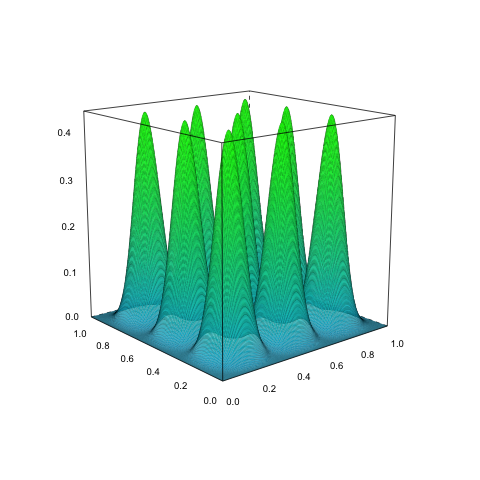
\includegraphics[width=4cm]{sparse_bicubic_basis}
% \caption{A ``thinned'' tensor product basis}
% \end{figure}
%     \end{center}
%\end{column}
%\end{columns}
%\vspace{0.3cm}
%\begin{equation*}
%\phi\left(l,m\right) = \sum_{i=1}^K \sum_{j=1}^L \theta_{ij} B_{i}\left(l\right) B_{j}\left(m\right)
%\end{equation*}
%
 
%The parameters of the functional autoregressive model given by \ref{eq:MyModel} define the elements of the precision matrix $\Omega$, rather than the elements of $\Sigma$ itself. It is well known that if we let $Y = \left(Y_1, \dots, Y_m\right)^\prime$ denote the random vector having joint distribution with mean zero and covariance matrix $\Sigma$, then the elements of $\Sigma^{-1}=\Omega$, $\left\{ \omega_{ij} \right\}$ may be interpreted as partial covariances between the elements of $Y$. This suggests shrinking $\phi$ to zero for large values of $l$. One can show that if $T$ has $k$ non-zero diagonals, then the middle $k$ diagonals of $\Sigma^{-1}$ are non-zero.  

%For ease of exposition, we first focus our attention on the estimation of $\phi$ assume that $\sigma^2\left(t\right)$ is fixed and known. Estimation of the innovation variance function is presented in Section~\ref{section:variance-estimation}. In the case that subjects share a common set of observation times $t_1 < \dots < t_m$,  it is well known that the MLE for $\Sigma$, $S = \sum_{i=1}^N y_i y_i^\prime$ is highly unstable in high dimensions, a condition that is potentially worsened when one or more subjects has at least one observation time that is unique from the set of observation times common across subjects. To mitigate instability due to high dimensionality and simultaneously permit the estimation of $\phi\left(\cdot,\cdot\right)$ as a smooth bivariate function, we obtain a covariance estimator by applying bivariate smoothing of the elements of the Cholesky factor. 
%
%Estimating the varying coefficient function $\phi$, however, is quite different from the usual problem of estimating an arbitrary bivariate function. In the case of the latter, we most typically treat both arguments equally in terms of regularization, but in the case of covariance estimation and the generalized coefficient function equal treatment of $l$ and $m$ in terms of penalization perhaps is not the most appropriate approach. The lag component, $l$, has particularly significant meaning in terms of the covariance function and thus also in terms of $\phi$ and is of considerable more interest than the orthogonal component, $m$. We parameterize $\phi$ in terms of the transformed domain:
%
%\begin{align*}
%l = t-s, \qquad m = \frac{1}{2}\left(s+t\right),
%\end{align*}
%\noindent
%so that the following relationship holds:
%\begin{align*}
%\phi\left(s,t\right) = \phi\left(s-t, \frac{1}{2}\left(s+t\right)\right) =\phi\left(l,m\right)
%\end{align*}
%with 
%\begin{equation} \label{eq:phi-star-domain}
%\frac{l}{2} < m < 1 - \frac{l}{2}, \quad 0 < l < 1.
%\end{equation}
%
%\noindent
%The likelihood can be written in terms of the reparameterized varying coefficient function:
%
%\begin{align} 
%\begin{split} \label{loglikelihood}
%-2L\left(y_1,\dots,y_N ,\phi \vert \vsigmasq \right) &= \sum_{i=1}^n \sum_{j=2}^{m_i} \sigma_{ij}^{-2} \left(y_{ij} - \sum_{k=1}^{j-1}\phi\left({t_{ij},t_{ik}}\right)y_{ik} \right)^2 \\
%&= \sum_{i=1}^n \sum_{j=2}^{m_i} \sigma_{ij}^{-2} \left(y_{ij} - \sum_{k=1}^{j-1}\phi\left({l_{ijk},m_{ijk}}\right)y_{ik} \right)^2 
%\end{split} 
%\end{align}

%%====================================================================================

\subsection{Model selection and tuning parameter estimation}

\subfile{chapter-2-subfiles/chapter-2-tensor-product-pspline-model-selection}


\bibliography{../Master}

\end{document}
